\chapter{Overview of Synthetic Data Generation}
\section{Overview}
In more broad and accepted terms, synthetic data is "any production data applicable to a given situation that are not obtained by direct measurement" according to the McGraw-Hill Dictionary of Scientific and Technical Terms. \cite{McGrawSyntheticData}\\ Synthetic data is not only popular and useful in computer science but it is also important in other business functions/types such as: Healthcare Systems, Fraud Detection Systems etc. In this project, the data synthesization of various real-life data stored into databases is important. In this type of data synthesization, that data is initially analyzed and then transformed, or rather just used in order to generate another set of data, so it isn't really a transformation but rather just a mere "sample" or "pattern" for the synthesized data.\\
\newline
Various methods and techniques are used in order to synthesize data. The procedure of this examination, analysis and generation of the real data into synthetic data is explained thoroughly and in more detailed and technical terms in the \nameref{ch:pgsynthdata_tool} chapter.\\
Synthetic data does NOT refer to anonymized data, it is often a misconception or a myth, there are various types of data transformations that can happen from real data such as: Anonymized data, artificial data, synthesized data etc. Moreover, there are also subtypes of the types mentioned above, which are of course, more detailed and technical. The image below by \citeauthor{Synthesized_2018}, depicts this in a pretty neat way.
\begin{figure}[H]
	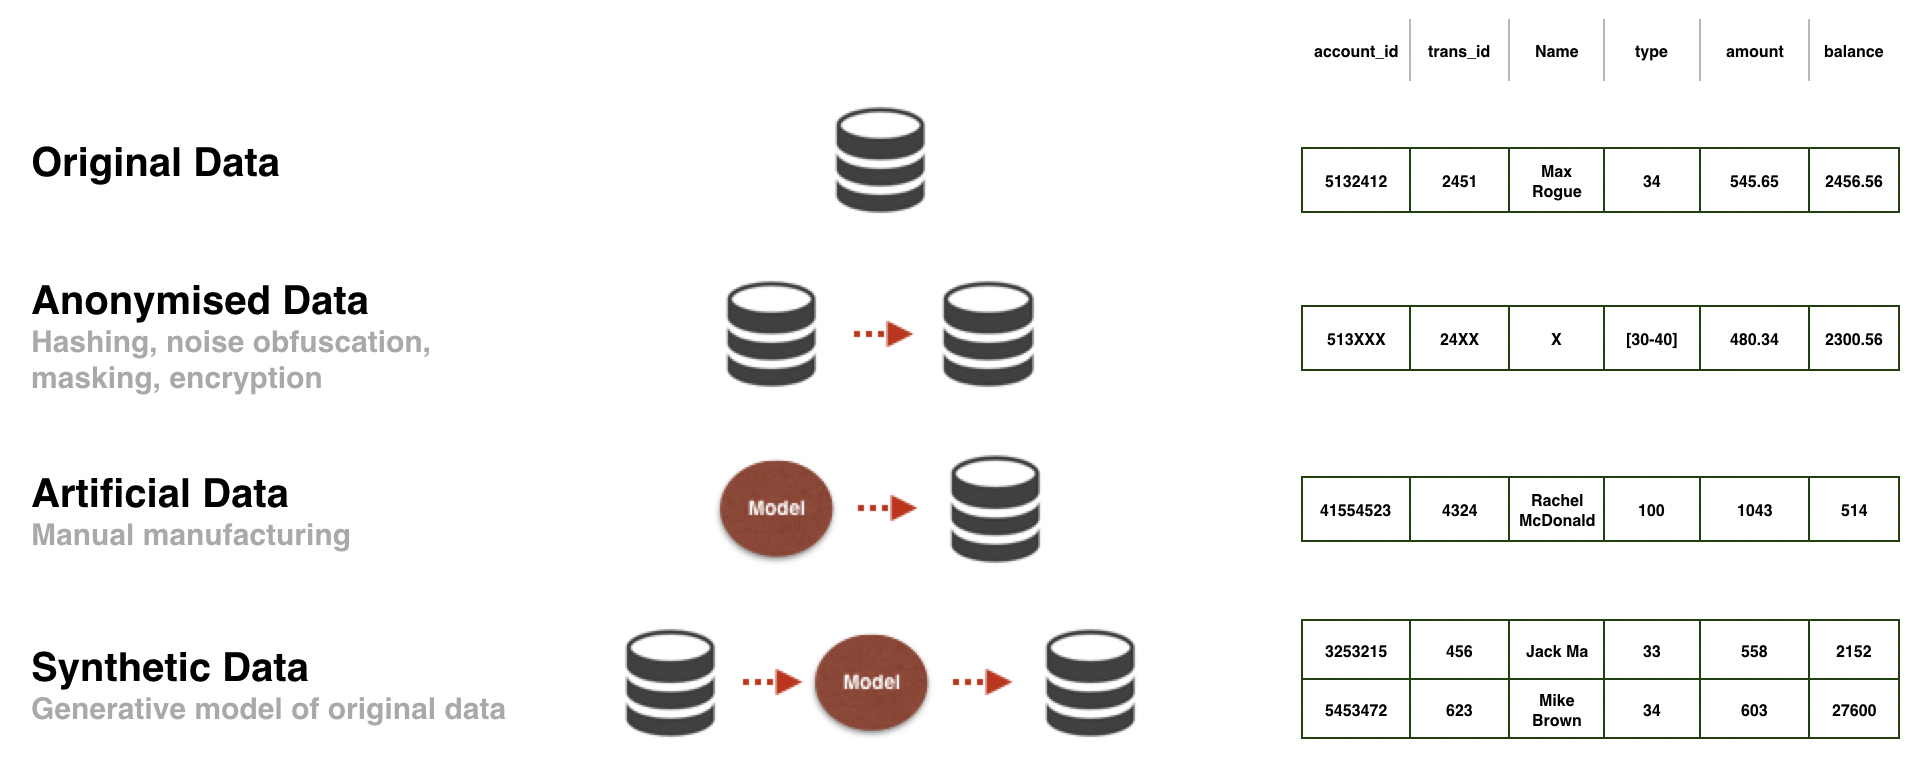
\includegraphics[width=\linewidth]{./Figures/Synthetic_Data/types_of_data_comparison.png}
	\caption{Three approaches to synthetic data, from \citeauthor{Synthesized_2018}}
\end{figure}
\newpage
\section{Data Synthesization}
Data synthesization is not a straight-forward process and it requires beforehand some sort of statistics and numbers that represent something. These statistics and numbers are then essential for the data synthesization process. The statistics must be correct and consistent so that the synthesization process can also be correct, with wrong statistics, we will get even worse results!\\
\newline
The statistics and numbers required for the synthesization are taken directly and only from the PostgreSQL database tables, especially from the \textit{pg\_stats} table. This table contains information such as: the most common values, what their frequencies are, the number of records that have NULL values, the histogram boundaries of the records, how distinct they are from one-another etc.\\
The \textit{pg\_stats} tables results, specifically, only the ones that the tool requires are first stored in a temporary dictionary and then read later in the data generation process. This information is transformed into Python objects and data types that are most convenient for the generation; manipulation done within this function is heavy. At the end of this function, objects with important and concise information are created, which are then used later for the actual generation/insertion of the data.\\
The synthesization process involves a lot of loops and arrays, and the data taken directly from the \textit{pg\_stats} table must be transformed into  information that is necessary for the further steps of the algorithm.
\section{Data Generation}
Data generation somehow falls under the data synthesization process, it only is a little more specific and is used for process abstraction. It may fall under a separate category too, but these concepts are still a little bit unknown and not clearly-defined by the community. For this tool though, the data generation part falls under the data synthesization process.\\
\newline
After the information has been retrieved from the database (the statistics and numbers) and stored into the relative objects, the data generation part begins.\\
In this part, the data is generated in an iterative fashion and then later inserted directly into the secondary PostgreSQL empty database. Data generated here, must be consistent and in conformance with the databases schema. If something fails here (at a column), usually, the whole table is skipped completely because the generation cannot proceed for that table anymore.\\
The generation process reads through every information that has been created previously and generates data by relying on that information. Some sort of manipulation is done here too, the information created before serves only as a "guide" for generating the data, and it is not the actual data itself.\\
The tool iterates through each column of the table and checks the data type of that column (which was added before), and then based on the data type, it does some operations that generate the data, always of course, relying on the \textit{pg\_stats} statistics. If the table/column have no pg\_stats available, data is generated regardless, however, it is generated in a fully randomized fashion because there is no statistics or numbers to rely on.
\section{Selected Database Related Open Source Tools}
TBD...
\section{Remarks and Further Resources}
TBD...